% !TEX root = ./First_year_report.tex

\chapter{Quantum Computing}
 
At a fundamental level, quantum computing is a discipline focused on developing hardware and software frameworks that leverage quantum mechanics to solve difficult problems. Whereas a classical computer uses information encrypted in elements called bits, taking values of 0 and 1, quantum computer elements can be in a superposition of states, and experience phenomena such as entanglement. The goal is to use quantum systems to solve computationally demanding problems more efficiently than the most powerful conventional computers. 

It is also worth mentioning that the work needed to achieve this has and will likely continue to contribute to our understanding of quantum mechanics and the development of new techniques in superconductivity, control of quantum systems and more. Due to this, progress in the field is important beyond short- or intermediate-term applications.

This chapter introduces the basic concepts behind quantum computing and provides a brief overview of the current state of the field. Afterward, the focus is on Quantum Error Correction, one of the main challenges behind this technology. Due to the nature of this project, the topics will be introduced from the well-known qubit-based perspective alongside the bosonic (quantum resonator-based) architectures.

\section{Fundamentals}
\subsection{The qubit and superposition}

The building block of quantum computation is known as the qubit or quantum bit. This concept is analogous to the more familiar bit, the smallest binary element in a classical computer. To establish a quantum information framework, the qubit can be defined in abstract terms as a two-level quantum system with possible states $\ket{0}$ and $\ket{1}$. This is an apt description of a variety of physical elements that can be used to build real computing systems, such as electron spins, photon polarization or superconducting circuits.

Due to its quantum mechanical nature, state $\ket{\psi}$ of a qubit is expressed as a superposition (linear combination) of states $\ket{0}$ and $\ket{1}$ as follows:
\begin{equation}
    \ket{\psi}=\alpha\ket{0}+\beta\ket{1}.
\end{equation}
Amplitudes $\alpha$ and $\beta$ are complex numbers obeying $|\alpha|^2+|\beta|^2 = 1$. It is possible to observe a bit and determine that its state is 0 or 1. In the case of a qubit in a superposition, an examination of its state gives less complete information. The outcome of the measurement will be $\ket{0}$ with probability $|\alpha|^2$ and $\ket{1}$ with probability $|\beta|^2$. Note that the properties of $\alpha$ and $\beta$ ensure that the probabilities of the states add up to unity.

The length 1 qubit states can be represented in a Block sphere, parametrizing the whole continuum of qubit states.
\begin{figure}
    \centering
    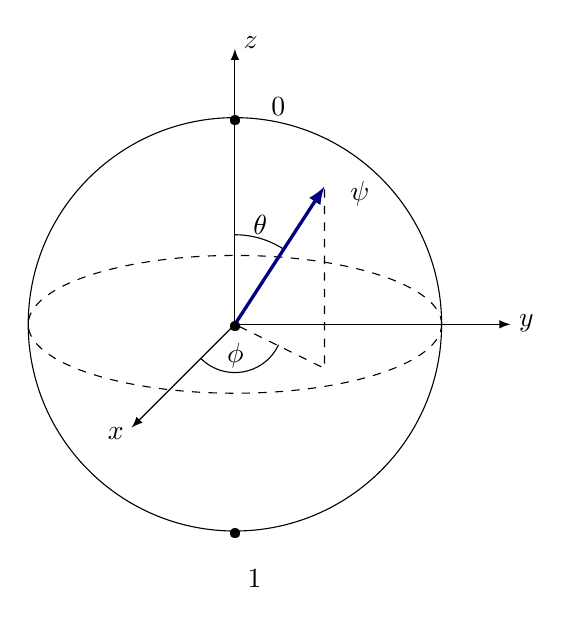
\begin{tikzpicture}[scale=1.75]
        \draw (0,0) circle (1.5);
        \draw[dashed] (0,0) ellipse (1.5 and 0.5);
        \draw[-latex] (0,0)--(2,0) node[label={[shift={(0.2,-0.35)}]$y$}]{};
        \draw[-latex] (0,0)--(0,2) node[label={[shift={(0.2,-0.25)}]$z$}]{};
        \draw[-latex] (0,0)--(-0.75,-0.75)node[label={[shift={(-0.2,-0.4)}]$x$}]{};
        \node[label={[shift={(0.55,-0.25)}]$\ket{0}$}] at (0,1.475){\textbullet};
        \node[label={[shift={(0.25,-1)}]$\ket{1}$}] at (0,-1.525){\textbullet};
        \draw[rotate=90] (0.65,0) arc (0:-33:0.65) node[midway,label={[shift={(0,-0.2)}]$\theta$}]{};
        \draw[-latex,NavyBlue,very thick] (0,0)--(0.65,1);
        \node at (0,-0.025){\textbullet};
        \draw[dashed](0.65,0.98)--++(0,-1.3)--(0,0);
        \node[label={[shift={(0.45,-0.5)}]$\ket{\psi}$}] at (0.65,1){};
        \draw[rotate=-135] (0.35,0) arc (0:110:0.35) node[midway,label={[shift={(-0.1,-0.2)}]$\phi$}]{};

    \end{tikzpicture}
    \caption[Bloch sphere representation of a qubit state]{Bloch sphere representation of an arbitrary qubit state (blue). Note how the orthogonal basis states $\ket{0}$ and $\ket{1}$ are shown as diametrically opposite.}
    \end{figure}
In the Bloch sphere, qubit states are represented in three-dimensional space in terms of two real parameters $\theta$ and $\phi$:
\begin{equation}
    \ket{\psi} =\cos \left(\theta /2\right)\ket{0} \,+\,e^{i\phi }\sin \left(\theta /2\right)\ket{1},
\end{equation}
with $0\leq \theta \leq \pi$ and $0\leq \phi \leq 2\pi$. Although at first glance it would appear there is an infinite amount of states that can be represented within a qubit. This however doesn't imply that an infinite amount of information can be encoded within it. Due to the quantum measurement phenomenon known as state \textit{collapse}, the outcome of qubit measurement will be either 0 or 1, providing one bit's worth of information. In fact, an exact determination of the parameters in a qubit state would require measuring an infinite number of identical qubits. At the same time, the properties of unmeasured qubits are essential to the power of quantum processing.

\subsection{Composite systems and entanglement}

Much in the same way as in classical computation, to carry out useful computations, several information units are needed. Therefore, it is essential to discuss how different qubits will interact with each other. When introducing a second qubit, the set of basis states will contain four elements, spanning all state combinations for both qubits: $\ket{00}$, $\ket{01}$, $\ket{10}$, and $\ket{11}$. The general state of the two-qubit system can be expressed as a superposition of the basis states, given by four complex amplitudes.
\begin{equation}
    \ket{\psi} = \alpha_{00}\ \ket{00}\ +\ \alpha_{01}\ \ket{01}\ + \ \alpha_{10}\ \ket{10}\ +\ \alpha_{11}\ \ket{11}
\end{equation}
Once more the squared norms of the amplitudes will represent the probability of measuring each state. Consequently, the state must be normalized according to $\sum_i |\alpha_i|^2 = 1$, for $i$ spanning all basis states. A measurement of this system could be applied to only one of the qubits, with a post-measurement superposition state conditioned on this outcome. For example, the first qubit will be measured at state $\ket{0}$ with probability $|\alpha_{00}|^2 + |\alpha_{01}|^2$. After obtaining this result, the system will be left in a normalized superposition of states $\ket{00}$ and $\ket{01}$.

An essential quantum behaviour that emerges when working with multiple qubits is the entanglement property, as best illustrated by Bell states (also known as Einstein-Podolsky-Rosen pairs). Consider the following superposition:
\begin{equation}
    \psi = \cfrac{\ket{00}\ +\ \ket{11}}{\sqrt{2}}.
\end{equation}
If the first qubit in this composite state is measured, the outcome will be $\ket{0}$ or $\ket{1}$ with respective probabilities of $1/2$. What is most interesting is what our measurement tells us about the state of the system overall. If the first qubit is in state $\ket{0}$ ($\ket{1}$), after measurement the system must be in state $\ket{00}$ ($\ket{11}$). Therefore, there is only one possible state the second qubit is allowed to be in, and gaining this information did not require performing a direct measurement. This shows how quantum elements can be correlated beyond what is possible for a purely classical system, and this property will be the basis of useful methods within the discipline of quantum computing. 

While discussing multi-qubit systems it is worth noting that for an $n$-state system, the basis states are simply a generalization of what has been discussed for the two-qubit case. It will once again be given by all possible combinations of qubit states. As a consequence the total number of encoded states grows quickly as $2^n$, achieving very high state numbers with qubit numbers in the hundreds. Due to the probabilistic nature of the qubits, it is possible to work with large amounts of quantum numbers simultaneously, far beyond what can be encoded classically.

So far, this section has focused on qubits as the essential units for quantum information. For the purpose of computation, however, the information must be manipulated as per the end goal. The next subsection discusses the gate operations that make this possible.


\subsection{Quantum logic gates}

In order to perform computations, bits and qubits, are used as part of computer circuits, in which information gets converted and transmitted. The operations to be applied can be as simple as the classical $NOT$ gate, which flips the value of a bit. If the bit is in state 0 it is changed to state 1, and vice versa. Logic gates can of course be more elaborate, for example, taking into account more than one bit.

Naturally, one must think of what gates must look like in quantum computers, taking into account knowledge of qubit states and quantum mechanics. The first key difference between a bit and a qubit is that the latter involves a linear combination of basis states. Therefore, a quantum logic gate needs to be able to act on this superposition state. To be compatible with quantum mechanics, and maintain the sense of probability, a quantum $NOT$ gate needs to be a linear operation.

Quantum logic gates are commonly expressed as matrices in the state basis. For the quantum $NOT$ case, the matrix representation is:
\begin{equation}
    X \equiv \begin{bmatrix}
    0&1\\
    1&0
    \end{bmatrix},
\end{equation}
where the first column and row correspond to state $\ket{0}$ and the second to state $\ket{1}$. Likewise, the qubit state can be represented as a vector in this basis:
\begin{equation}
    \ket{\psi}=\begin{bmatrix}
    \alpha\\
    \beta
    \end{bmatrix}.
\end{equation}
Then the quantum $NOT$ gate acts on the qubit as:
\begin{equation}
    X\ket{\psi} = \begin{bmatrix}
        \beta\\
        \alpha
        \end{bmatrix},
\end{equation}
flipping the amplitudes associated with each basis state.

Linearity is not the only property of quantum mechanical systems that must be reflected in quantum logical gates. As was mentioned previously, the probabilistic nature of qubits requires states to be normalized. This must be true before and after a logic operation is applied to the qubit (probability must be conserved). Therefore, any $2\times 2$ matrix $U$ associated with a quantum gate must be unitary, obeying
\begin{equation}
    U^\dagger U = I,
\end{equation}
where $I$ is the $2\times 2$ identity operator.

The properties of linearity and unitarity generalize for gates acting on multiple qubits. One useful example of this is the two-qubit CNOT gate (also known as controlled $NOT$):
\begin{equation}
    CNOT=\begin{bmatrix}
        1&0&0&0\\
        0&1&0&0\\		 		
        0&0&0&1\\
        0&0&1&0\\
    \end{bmatrix}
\end{equation}
This gate performs a $NOT$ operation on the second qubit, as conditioned by the state of the first qubit (which is left unchanged). The effect of this gate is summarized in the following table:
\begin{table}[hbt!]
    \centering
    \begin{tabular}{l | c }
        IN & OUT\\
        \hline \hline
        $\ket{00}$ & $\ket{00}$ \\ 
        $\ket{01}$ & $\ket{01}$\\
        $\ket{10}$ & $\ket{11}$\\
        $\ket{11}$ & $\ket{10}$
    \end{tabular}
\caption{$CNOT$ gate truth table}
\end{table}
\FloatBarrier

The equivalency between the $CNOT$ gate and a classical counterpart is not as direct as what can be drawn between the classical and quantum $NOT$ operations. This is due to yet another useful property stemming from the quantum nature. Quantum logical gate representations are always invertible, meaning that their effect is reversible. Meanwhile, the classical analogue to the $CNOT$ operation ($XOR$ gate) loses information, and therefore the state before its application cannot be recovered.

 It is worth mentioning as well that the conditional action based on the state of the first qubit does not constitute a measurement. Due to this, it does not cause a collapse of the superposition state, making the $CNOT$ gate an extremely powerful tool. In fact, it is proven that the use of $CNOT$ gates alongside the set of single-qubit rotations is sufficient to perform any operation (on any number of qubits). This is known as universality, and can theoretically be realized to arbitrary accuracy.
 Another aspect of note is that the $CNOT$ gate can be used to prepare entangled states, such as the aforementioned Bell states.

\section{Current Capabilities}

\subsection{The NISQ era}
Presently, quantum computing is in its NISQ era, standing for (Noisy Intermediate-Scale Quantum). This denomination refers to some of the main challenges of quantum computation. 

The first challenge is noise. Even within the context of classical computing, there exists a possibility of random errors that may modify the state of one or more bits. The quantum properties of qubits make them particularly susceptible to environmental interference. As was discussed previously, an interaction (or measurement) will lead to quantum decoherence, and so eliminate the useful characteristics of the system. Due to this, hardware implementations need to put special emphasis on, for example, isolating qubits and preventing thermal fluctuations. 

Another way of approaching noise mitigation is implementing error correction algorithms, which can identify and rectify issues that arise. Executing these algorithms, however, necessitates using more qubits in a given calculation. This leads to the second challenge of the NISQ era: the intermediate scale. This refers to the size of the quantum systems that can actually be realized in hardware. The size or volume is thought of in terms of qubit number and number of applied gates. In a circuit comprised of qubits with some probability of failure, the probability of having some error increases with the qubit number. Likewise, whenever a gate is applied there is some probability an error will be caused, so the overall probability of error increases the more we operate on the system.

Recent work by several companies (such as IBM, Rigetti, and Google) has enabled great strides in the number of qubits of current quantum systems, which in the last few years has jumped from below 50 to around 1000 qubits. In the short and intermediate term there is still plenty of work to be done to not only allow for the increase of this number, but also ensure higher coherence times, more accurate gate operations, and more efficient error correction algorithms. These are some of the elements that will come into play in the development of fault-tolerant\footnote{Fault tolerant systems can continue functioning adequately even if some errors or partial failures are present.} quantum computers and the achievement of quantum advantage\footnote{Quantum advantage refers to conclusively proving that a quantum computer can solve a problem that no classical computer can solve within a reasonable timeframe. Computationally complex problems can often be theoretically computable classically, however, due to exponentially increasing timeframes may only be achieved at time scales beyond human interest.}.

The basic ideas behind Quantum Error Correction, along with some examples, will be addressed in a later chapter. The next subsection provides an overview of some of the physical systems that are currently used as quantum hardware.

\subsection{Hardware approaches}

As was described in the previous subsection, the quantum computing framework can be carried out through different physical systems. These include, for example, superconducting qubits, trapped ions, and photonics. The following descriptions do not aim to provide a comprehensive overview of each hardware architecture, and instead hope to provide a more grounded idea of how quantum computing is carried out. As will be described, each hardware implementation presents a set of limitations that need to be addressed to develop usable quantum computers. At the same time, each of them can also provide unique advantages and can be worked with from different conceptual points of view. 

Perhaps the best-known type of quantum hardware is based on superconducting qubits. These systems build qubits from Josephson junctions, formed by two superconducting elements separated by a fine insulator layer. Due to the Josephson effect, this junction will allow a current between the superconductors, enabled by \textit{quantum tunnelling}\footnote{Quantum tunnelling is a quantum mechanical effect that allows particles to go through barriers (such as the walls of a potential well), despite their energy being lower than that needed to surmount them according to classical physics.}, thus displaying a quantum effect at a macroscopic scale. The logical qubit states $\ket{0}$ and $\ket{1}$ can be mapped to different physical states of the superconducting components, such as discrete energy levels. The elements are then arranged into a circuit. 

In order to manipulate these superconducting circuits to perform computations it is necessary to construct reliable control operations. In the case of superconducting qubits, microwave pulses can be administered to execute single-qubit or multiple-qubit gate operations. The control and readout of the superconducting qubits are carried out using classical computers, that are already built for user interfacing.

Due to their superconducting nature, these systems need to be maintained at cryogenic temperatures to prevent decoherence. The cabling linking circuit elements and aspects such as qubit readout also need to be optimized to minimize incidences of errors and allow for the scalability of the systems. In other words, technical advances in hardware development are essential to building quantum computers with larger qubit numbers that can execute more gate operations, while avoiding the exponential increase of errors. Some of the companies focused on this task are Rigetti, IBM, and Google.

Computation using superconducting qubits does not always rely on gate operations. This is the case in quantum annealers, such as those developed by D-wave. These systems apply magnetic fields to superconducting qubits that can manipulate the probability of a qubit being in each state (bias). Lattice configurations are assembled for these qubits, establishing couplings between them with arbitrary correlation weights. A user choice of qubit biases and couplings can be used to solve optimization-type problems. The annealing process consists of slowly evolving the system from a ground state of unbiased and uncorrelated qubits into the ground state of the problem that the user desires to solve.

A classic case of an optimization problem is that of the travelling salesman. The goal of the problem is to find the shortest route for the traveller between a set of towns. Although coming up with a classical algorithm to solve this problem is straightforward (simply calculate distances for all possible paths and compare), its computational cost increases exponentially with the number of towns. Thus, the problem cannot be solved by classical computers for non-trivial cases (although heuristic solutions exist which provide approximate solutions for some more complex cases).

This is the type of problem that could benefit from a quantum annealing-based computer. In this case, the correlations between qubits represent the distances between the cities. Meanwhile, the qubit states contain the information on whether a town was (or wasn't) visited in a sequence step. The total system energy for a given state is associated with the distance traversed by the traveller if the towns were visited in that particular order. Thus, the ground state provided by an annealer will correspond to the desired solution, the optimal path. It is worth noting that this approach is also liable to qubit decoherence, as well as other sources of error. Furthermore, the annealing process can be heuristically transposed into gate-based quantum computers to address optimization problems.

A third type of quantum computer is the bosonic system. This dispenses with the focus on two-level qubits. Instead, bosonic computing's basic unit is the qudit, which can have N levels. In physical terms, a qudit is implemented using a quantum harmonic oscillator, and assigning a logical state to each of its accessible energy levels. Quantum oscillator systems can be built using Superconducting radio-frequency (SRF) cavities, which have very low rates of dissipation and are therefore well equipped to maintain state coherence. 

The ability to encode a higher number of states within one single hardware element is key to implementing Quantum Error Correction procedures without introducing new sources of noise. The possible errors in a resonant cavity are linked to photon loss, which is easy to detect and correct. These advantages have turned bosonic platforms into an area of high interest and expectation. As bosonic quantum computing is a focus of this PhD, a further section will be dedicated entirely to this particular topic.


\section{Bosonic Systems}
\textcolor{red}{Reassess whether this is better off here or after the section on Quantum Error Correction.}

\vspace{5cm}
Qubits, NISQ overview: \cite{Nielsen2010} \cite{Preskill2018} \cite{IBMintro} \cite{Kaye2007} \cite{Cleve2021}. 
Expected applications (brief), perhaps better suited to the intro section?

Different hardware approaches (brief): \cite{Dwave} \cite{Zurich} \cite{IBMtec}

Bosonic systems: \cite{Zurich} \cite{Girvin2021}, cQED

\clearpage
\section{Quantum Error Correction}

As was established in prior sections, quantum computers are susceptible to environmental noise which jeopardizes the coherent states containing information. The field of error correction is well-established for classical computers. However, classical corrections algorithms cannot simply be applied to quantum systems. Qubits, unlike bits, are limited by the no-cloning theorem, stating that it is not possible to make independent, perfect copies of a qubit's state. There is also the problem of quantum measurement and wavefunction collapse. Despite this, Quantum Error Correction (QEC) is a productive field of study, and many viable approaches to error mitigation have been proposed. The following section aims to introduce the fundamental ideas behind QEC at the qubit level and the bosonic level, alongside some example implementations.

\subsection{Introduction to Error Correction}

One of the basic ideas behind error correction is that of redundancy. In simple terms, it consists of using a higher number of bits (or qubits) to encode one bit (or qubit) of information. A simple illustrative example is that of the classical repetition code. Instead of just utilizing one bit with possible values of 0 and 1, one can define logical codewords. These logical codewords are strings of multiple bits, mapped to logical states 0 and 1. For the three-bit repetition code, codeword '000' (three bits in state 0) corresponds to logical state 0, while codeword '111' does to logical 1. 

In classical computing, there is only one possible error, known as bit flip. A bit flip occurs when a bit in 0 gets mapped to 1, or vice versa. When transmitting the logical states, the receiver could get '100', '010' or '001' instead of codeword 0, assuming only one bit flip occurs. This error can easily be remedied using \textit{majority voting}. Simply put, if most of the bits take value 0, the 1-valued bits are assumed to have flipped, and the error can be rectified. 

If two bits happen to flip, the error can be detected, as the transmitted bit string does not match either codeword. However, this error cannot be corrected using majority voting, and the received logical bit will be incorrect. If three errors occur, the situation is even more dire, as the resulting state is still a valid codeword, and the error cannot be detected, much less rectified. This does not mean that the three-bit repetition code (despite being inefficient) is unable to provide any improvement. Error correction is based on the assumption that hardware performs well enough that errors are rare. Thus the goal is not to provide ideal error correction, but to further reduce the already low incidence of errors. In the case of the three-bit repetition code, low error probabilities mean that uncorrectable errors (two or three bit-flips) are significantly less likely than the correctable single bit-flip. Likewise, undetectable errors are the least likely to occur. 

It is worth noting that some tools to address errors can be designed with only detection (and not correction) in mind. For example, for an arbitrary bit string, an additional bit can be implemented to record the string (plus ancilla) parity. This is achieved by mapping even and odd parity to 0 and 1. If at a later stage the parity of the new bit string is odd, an odd number of bit-flips must have occurred. The exact details of the errors cannot be obtained from the bit string, but the string is known to be corrupted. Given that the incidence of no-flip and one bit-flip events is much higher than that of two bit-flips (where parity is indistinguishable from the errorless case), it is reasonable to assume that an even parity implies that no bit has flipped. Likewise, it is to be expected that an odd parity was caused by one single error.

When adding ancilla bits, it is important to consider that the error rate is a priori increased. Consider once again the repetition code. If each bit in a certain hardware system is known to have a probability of error $\epsilon$, the probability of having no errors on a bit is: \begin{equation}
    P_0=1-\epsilon.
\end{equation}.
Once the ancillae are introduced, this becomes:
\begin{equation}
    P_0=(1-\epsilon)^3.
\end{equation} 
Therefore, the probability of at least one error occurring is 
\begin{equation}
    1-P_0 \sim 3\epsilon,
\end{equation} 
tripling that of the single bit (in the small $\epsilon$ limit). Thus, a successful error correction code must surpass the break-even point: the logical (error-corrected) bit error rate must be lower than for the physical bit. 

Consider the break-even point for the repetition code. The logical bit error rate is given by the probability of running into an uncorrectable error (having two or three bit-flips). This can be expressed as:
\begin{equation}
    \epsilon_{logical} = P_2 + P_3 = 3\epsilon^2 - 2\epsilon^3.
\end{equation}
Probabilities $P_2$ and $P_3$ correspond to the two and three bit-flip cases respectively. For this case their values are $P_2 = 3\epsilon^2(1-\epsilon)$ and $P_3 = \epsilon^3$.

The breakeven point equation $\epsilon_{logical}=\epsilon$ shows that the repetition code will reduce error occurrences for physical bit error rates below $1/2$. The form of $\epsilon_{logical}$ also shows that, as expected, logical bit error rates decrease with physical bit error rates.

It is worth noting that introducing error correction for bit flips does not provide complete fault tolerance, as more realistic error models need to take into account errors introduced when other system elements fail. This includes accounting for possible errors in the error-correction circuitry itself or errors attributed to the process of measuring bit states. For example, a realistic logic gate will have some chance of failing when used. The goal is to design error correction circuits that only incur errors that it can detect and correct in its subsequent applications.
This also affects the frequency at which the correction process must be applied.

If there is a certain probability of each bit in the system flipping in a given time interval, a repetition-code-based correction scheme needs to be applied before the probability of uncorrectable errors becomes too large. However, if the correction code is applied too often, there is a risk of having error correction circuit errors (such as incorrect majority voting). Near-perfect correction circuits should enable fault tolerance through speedy circuit implementations. However, realistically, the delay between operations will be affected by the take to execute.

Having discussed some of the basic concepts and motivations when performing error correction, let us move on to applications to qubit-based systems.


\subsection{Error correction for qubit systems}


\clearpage

General \cite{Girvin2021} \cite{Andersen2020} \cite{Gottesman2009} \cite{Roffe2019} \cite{devitt}

Specific Implementations \cite{Krinner2021} \cite{Chen2021} \cite{cleland2022}

Bosonic \cite{campagne2020} \cite{Lau2016} \cite{Chuang1997} \cite{Terhal2020} \cite{Blais2020} \cite{Hu2019} \cite{Michael2016} \cite{Grimsmo2021} \cite{Cai2021} \cite{Brady2023} \cite{lachance2023}